% !TeX root = ../main.tex
\documentclass[./../main.tex]{subfiles}

\begin{document}

\subsection{Thiết kế bậc cao}

Hệ thống có 5 thành phần chính:
\begin{enumerate}
	\item Web Client: dành cho người dùng máy tính.
	\item Mobile App: dành cho người dùng di động.
	\item Server: Cung cấp API để client hiển thị.
	\item Cache Server: lưu trữ các dữ liệu được truy cập nhiều. Cụ thể, cache lưu lại các token bị blacklist.
	\item Database: lưu trữ thông tin về các thực thể trên hệ thống.
\end{enumerate}

\begin{figure}[H]
	\centering
	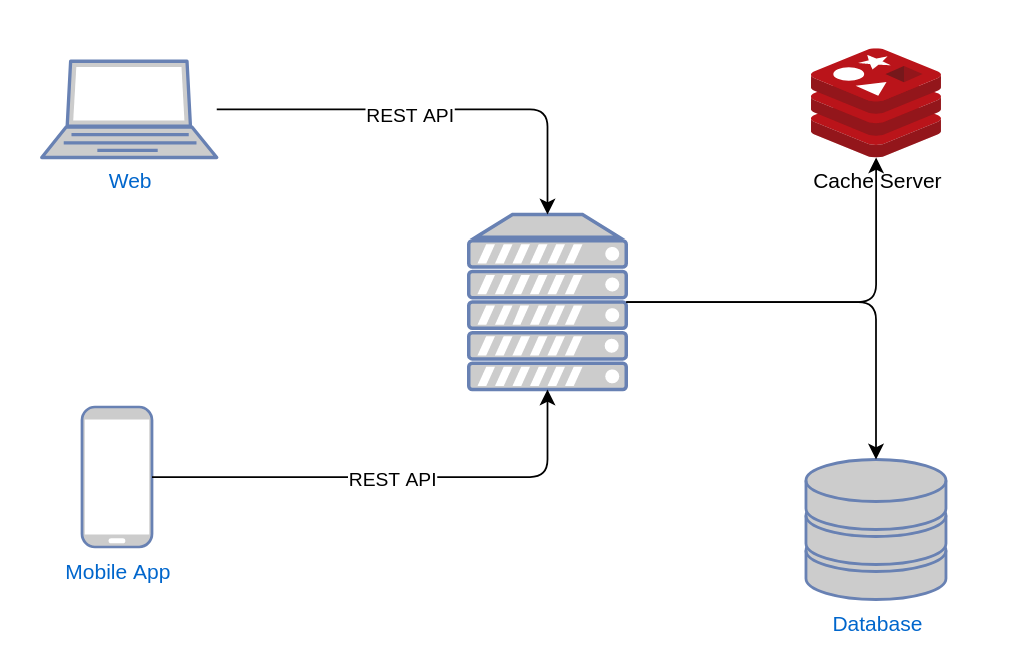
\includegraphics[width=\linewidth]{./images/high_level_diagram.png}
	\caption{Biểu đồ thiết kế bậc cao}
\end{figure}

\subsection{Thiết kế API}

API của hệ thống được thiết kế theo chuẩn REST để dễ dàng sử dụng. Tài liệu về API được lập trình viên backend tạo và upload lên \url{https://honyomi.stoplight.io/}.

\subsection{Thiết kế cơ sở dữ liệu}
Dù nhóm quyết định sử dụng cơ sở dữ liệu NoSQL dạng Document-base nhưng các lược đồ của cơ sở dữ liệu vẫn được nhóm xây dựng dựa trên mô hình thực thể - quan hệ (ER).
\begin{figure}[H]
	\centering
	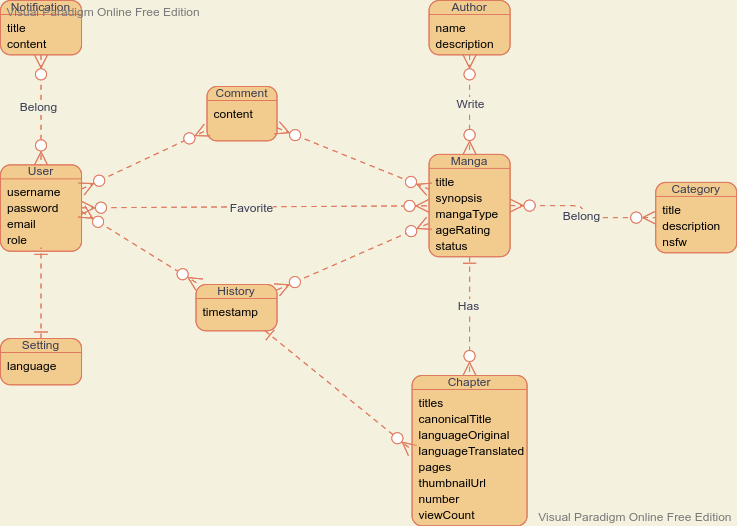
\includegraphics[width=\linewidth]{./images/image8.png}
	\caption{Biểu đồ thiết kế cơ sở dữ liệu}
\end{figure}
Dựa vào phân tích ER trên, các lược đồ được sinh ra sẽ gồm các Document sau:
\begin{itemize}
	\item User: lưu thông tin và cài đặt của người dùng.
	\item History: lưu lịch sử đọc truyện của người dùng.
	\item Favorite: lưu danh sách yêu thích của người dùng.
	\item Manga: lưu danh sách truyện trên hệ thống.
	\item Chapter: lưu danh sách chương truyện.
	\item Category: lưu thể loại truyên.
	\item Author: lưu danh sách tác giả.
\end{itemize}
\end{document}
